\chapter{空想統計教程}
本書は統計学を使って科学的な推論・予測を行うプロセスを説明したものである。
ただし、このプロセスを通して研究を行っている人は少なく、認められていない方法である。
ゆえに本書が説明する全ては、空想である。
なぜこのような空想が必要であるのかを本章で説明する。

%私が知りたいことを知るためにどのような統計量が必要なのかを説明している。

\section{生物統計学の問題点}
一般的な生物統計学の書籍には、論文を査読プロセスに耐えるための方法論が記載されてる。そのため、生物学の各分野に特化したものが多く、それぞれ独自の特徴を持っている。
例えば、以下が問題がある。

\begin{enumerate}
 \item 繰り返し検定を行っていき、最終的な検定方法を決定する。いわゆる検定フロー
 \item $p$値のさまざまな解釈間違い
 \item 統計モデルとデータの比較で言えそうにないことまで言う。
 \item $p<0.05$であるので対立仮説を採択する。
 \item 何のために行っているのか不明な解析
\end{enumerate}
これらの特色は統計を理解している科学者から否定的に批判されており、生物学者たちもよく理解していると考えられる。しかし、なぜこれらの特色が使い続けられているのだろうか?

一般的に、生物統計学の書籍を執筆するのは、多くの論文を学術誌に投稿し、掲載された研究者たちである。掲載には2人程度の査読者が割り当てられ、論文を査読され、そこで使われている統計がその学術において妥当であるかどうかが調査される。この査読プロセスに耐えられるように統計を使うことが必要であり、その経験を元にして一般的な生物統計学の書籍が執筆されているのだと考えられる。

ただし、このような目的が論文の掲載になっているため、科学的に何をすべきかを考えることは二の次になってしまっているのではないだろうか。


生物統計学の本では、$t$検定を行う前に正規性の検定を行うことを求めているものが多い。正規性の検定を行っても、サンプルが正規分布から抽出されたかどうかを確認できないから、生物統計以外では推奨されていない方法である。

もし正規性の検定を行わないことが査読プロセスで要求されているなら、正規性の検定を拒否した著者の論文は出版されにくくなると予想される。Publish or Perishの世界において、論文が出版されなければ、その研究者のキャリアは短命となることが想像できる。

一方で、業界内で認められた統計解析を行い、その結果に基づいて論文を出版した研究者は、研究者としてのキャリアを築いていくことができる。このような研究者は、査読プロセスで得られた知見を元に、その業界内での適切な解析方法を学び、その後、生物統計学の本を執筆することなる。
言い換えれば、推奨されない方法を学んだ科学者は生き残りやすく、そうではないものは生き残りにくいというバイアスが働きやすくなる。

%生物統計学においては、妥当とされる方法論も、常に見直しと改善の余地があることを忘れずに、書籍を執筆することが重要である。





%editorや査読者ではなく、自然をよく予測できるかどうかであるだろう。
%そのために必要となるデータや指標・統計量は何かを理解する必要がある。
\if 0
帰無仮説を否定すれば、対立仮説を採択するというのも、生物統計の特色である。
言い換えると、イコールの仮説では$p<\alpha$だったから、イコールではない仮説が成立すると生物統計学では主張できる。
この考えは本書では推奨しない。
イコールでない仮説についてなんら検証できていないからである。
\fi





\section{生物統計学と本書の違い}
以下には生物統計学の書籍と異なる点を示す。

\subsection{ASAの$p$値に関する解釈}
$p$値に関する解釈は、アメリカ統計協会(ASA)が2016年に発表した声明に従う\cite{doi:10.1080/00031305.2016.1154108}。以下に引用しておく。
\begin{quote}
 P-values can indicate how incompatible the data are with a specified statistical model.
\end{quote}
日本計量生物学会が公開した翻訳では、
\begin{quote}
 $P$値はデータと特定の統計モデルが矛盾する程度をしめす指標のひとつである。
\end{quote}
この翻訳された文章ではincompitableを矛盾としている。本書では適合と翻訳する。
日本語の翻訳を書き換えると、$p$値は、データと特定のモデルの適合を示す指標の一つである。
データとモデルの適合とはどういう意味なのかを後で定義する。

%この声明に従った生物統計学の書籍は少ない。

ASAが$p$値をどのように使ってほしいと考えているかについて関係者ではない私は理解していない。ASAの発表を私の都合に合わせて使っているにすぎない。
また、ASAの解釈を採用している生物統計学の書籍は非常に少数である。

\subsection{仮説検定}
生物学的問いからある2数の生物の計測可能な特徴量に関する予測を立てる。
その予測とは以下のようになる。
%初等的な生物統計学の書籍に提示されているのは、
\begin{enumerate}
 \item OO条件とXX条件では~という特性に$\cdots$という差がある
 \item A群とB群の特徴量の平均値が異なる
 %\item A群とB群について平均値に差があるか
\end{enumerate}
現在の生物統計学においては、これらの問いを有意差検定を用いて解決を試みている\footnote{失敗している}。
具体的には、母数が同一のモデルを仮定し、そのモデルにデータが適合するかを検証する。
適合していなければ、母数が異なると判定をくだしている。
このような扱いは本書では推奨しない。
本書ではこのような方法によってわかることは、検定統計量について適合しなさそうなモデルが明らかになった。
これよりも多くのことを、有意差検定であきらかにはできない。

本書では、これらの問いについてA群とB群に共通する特徴について、その特徴を測定した標本が適合するモデルをそれぞれの群に対して特定する。
さらに、それらのモデルの性質の違いを明らかにする。
ここまでが本書で扱う内容である。
生物学ではさらに、それらの適合モデルの違いが生物学的にどのような影響をもたらすのかについて考察する必要がある。
この点は、本書で扱っていない。


\subsection{仮説検定とモデル選択}
$p$値を使ったモデル選択は、仮説検定と数学的に同じである。あるモデルにおける統計量の統計的性質を用いてモデル内でのデータを元にした統計量以上の値が出現する確率が$p$であり、仮説検定とモデル選択は同じ作業を行なっている。
%あえて言えば、モデル選択と名乗っているが、$p$値を使っているモデル選択は、モデル非選択といった方が良い。
%\section{データが汚いので予測は手順を踏むだけ}

%言い換えるならば、統計学を使って一般のことについて推測しやすいデータを得られたときに言えることを学ぶことで、より難しいデータが得られたときに、言ってはいけないことを学ぶべきだろう。
\subsection{頻度論}
\begin{defi}
頻度主義とは次のこととする\cite{efron2020大規模計算時代の統計推論}。
  \begin{quote} ある計算手続を決めたとき、その確率的性質を導き、観測データに対して計算手続きを行って得た出力に、導いた確率的性質をそのまま適用する。
  \end{quote} 
\end{defi}

%頻度主義は、繰り返し試行を行った結果得られる統計的性質を、そのまま観測データに当てはめる。扱う問題は、次のようなものである。
頻度主義において、データがある分布関数に従っていることを前提とし、その母数を推定することが初等的な問題設定となる。
扱う問題として、次の様なものがある。
\begin{quote} 大量に生産された製品の中から無作意抽出された製品に関するデータについて、そのデータの平均値と母標準偏差があたえられているとする。このとき、このデータの平均値を用いて信頼区間$95\%$で母平均を推測することなどに統計的な推測の考えは活用できる。\footnote{\url{https://www.stat.go.jp/teacher/dl/pdf/c3index/guideline/high/math.pdf}}
\end{quote}
これまでの計測および解析により分布形が明らかになっていることを前提として、少数のデータからその分布形を推定することに利用されている。

一方で、生物学においては、分布形の前提が常に確定しているとは言い切れないので、分布形推定からおこなうことになる。
さらに、頻度主義で行われている確率的性質を観測データにそのまま適用し、解釈するということは、生物学においてそのまま適用するしばしば不適切な解釈となる。

前提の見直しは頻度論の教化書では扱うことが少ない\footnote{生物統計学の教化書では、正規性の検定を行うことになっていが、検定をしてもそのデータが正規分布に従うとは言えない。}。
本書では、頻度論統計学の知見を元に、頻度論が対象にしていない範囲で推論を行う方法を説明する。
具体的には、正規分布で予測できることがわからない対象に対してモデルを構築する考え方と推定方法について説明する。
さらに、頻度主義で明かになっているモデルの性質を用いて、そのモデルのデータへの適応の妥当性について議論する。
そのとき、議論かのうとなる事柄について整理していく。

\begin{SMbox}{「数理科学を使えば統計の”主義”を争う必要ない」}
 \begin{enumerate}
  \item 「“数理的な方法”を使っても、主義の争いが解決しない」ということを示唆する事実が存在する
  \item 頻度主義とベイズ主義の論争を「どちらの方法が正しいか」という争いとして捉えると論争の全体像を見誤る
 \end{enumerate}\footnote{「数理科学を使えば統計の”主義”を争う必要ない」という主張について検討する\url{https://ameblo.jp/yusaku-ohkubo/entry-12588890730.html}}

\end{SMbox}

\begin{SMbox}{生物統計学では言えないことも言える}
統計学を使っても主張できないことを生物統計学では主張していることが多々ある。
この理由を探そうとしても大抵徒労に終わる。
生物統計の解析手順いわゆる検定フローをやってるだけである。
ある統計処理をしても判定できないことを判定できることにして処理を進めていることが多い。
%ただし、生物統計が扱うのは頻度論では扱えない範囲なので、統計学では言えないことでもある程度認めなければいけない事項がある。
\end{SMbox}


\begin{SMbox}{生物学部の卒論発表会に登場する統計学者}
 生物学部の卒論発表会に、統計学を学んだ先生方が登場することがある。彼等は、卒論生の発表をきき、検定フローに従って作業を行っていないばあ、厳しく叱咤していく。例えば、この検定を実施する前に、検定の仮定について検定しているのか?していないなら、この結果を信じることができないなど。
 生物学の先生は、統計学の先生に御礼を言い、そのおかげもあり、次の年も統計学の先生が学生たちを叱咤しに卒論発表会にくる。
 統計学の先生が行っていることは本当に良い行為であろうか?彼らの言うことを聞いていれば、我々にとって知りたいことがより理解できるのだろうか。

 この統計学の先生は、日本以外にも出没しているように思える。
 \begin{quote}
  A lot can go wrong with statistical inference, and this is one reason that beginners are so anxious about it. When the framework is to choose a pre-made test from a flowchart, then the anxiety can mount as one worries about choosing the “correct” test. Statisticians, for their part, can derive pleasure from scolding scientists, making the psychological battle worse.
 \end{quote}\footnote{Statistical Rethinking 2nd Edition Chapter.1 P.4より}

\end{SMbox}

\chapter{モデル}
モデルについて説明する。

\section{モデル}
モデル(模型)は次の特徴を備えている。
\begin{enumerate}
 \item モデルは本物の特徴の一部を推測可能。本物との乖離の程度も推測できる
 \item 複数の仮定により構築される。また、それらの仮定は、現状の知識では明らかではないまたは、現実的には成立していないことがある。
       %推測可能なことを増やすために仮定を増やすことがある。
 % \item モデルは本物の要素・特徴の全体を推測することはできない。
 \item モデルは間違った推測をする。
\end{enumerate}
  
例えば、車のプラモデルはモデルである。本物の特徴の一つである大きさを推測可能にするため、スケール(例えば、1/24など)を決めて作られている。車体の幅などを計測し、スケール倍すれば、実物の大きさを推測できる。
手のひらに収まるような小さなプラモデルでも、スケールが同じであれば、どの部分でも実物と同様に推測することができる。
つまり、本物の車がなくても、スケールが合ったプラモデルがあれば、簡単に大きさを推測することができる。
言い換えれば、実測した数値をモデルに組み込むことで、推定の精度を上げることができる。

車がもっとも正確なモデルと言えるが、実際に車を用いて様子を推測することは、手間がかかりますし、モデルの利便性を損なう。また、細部まで推測可能にするためには、より高精度の測定器具が必要になるため、モデルとして利用する際のデメリットになることがあります。

モデルは、推測したい内容に応じて構築されるため、完全に現実を再現する必要はありません。例えば、同じ車を3台縦列に駐車するために必要な長さは、単純な直方体3つ分で推測できます。そのため、車のモデルには大きさの尺度を保っていない直方体のブロックを使用することがあります。

モデルは対象としていなかったものについても予測できる。例えば、軽自動車の大きさを予測するモデルを使ってトラックの大きさを予測することができるが、その予測値は実際のトラックの大きさと異なる。モデルが車体長を3.4mと予測した場合、実際のトラックの車体長は6mよりも大きいこ。つまり、メートル単位でモデルと実際との差が生じている。

このように、モデルと実際を比較することで、このモデルではトラックの大きさを推測できないことが判明することがある。ただし、実際にどの程度の誤差が生じた場合に、そのモデルが使えないと判断されるかは、予測したい内容によって異なる。

%モデルは本物ではないが、推測に役にたつ物として利用する。モデルと本物が極めて一致するように感じられることもあると思うが、モデルは本物ではない。

\section{統計モデル}
%統計モデルについて説明し、モデルを使って現実を推測することを概念図を用いて説明する。
まず、統計モデルは数理統計の知識を用いて構築され、現実を推測するために使用される。例えば、以下のような仮説から構築される簡単な統計モデルがあります。

\begin{enumerate}
 \item (仮定1)確率変数が同一の分布から独立に得られる(i.i.d)
 \item (仮定2)その分布関数は、$f(x)$で表される
 \item (仮定3)分布関数の母数に関する仮説\footnote{なお、中には三番目の仮説のみを統計モデルと主張する学派もある\cite{塩見_正衛2021}}
\end{enumerate}

\begin{comment}
% https://twitter.com/ibaibabaibai/status/1702697352258359564
 今日も酔っ払った勢いでいっぱい話したけど、モデルというのは世界をどのように見るかであって、真なる世界の話はしてないってのをみんなもっと考えてほしいな!
 線形モデルが正しいとかではないのよ!我々はどう見るかなの!

% https://twitter.com/ibaibabaibai/status/1702697896746131637
 「モデルというのは世界をどのように見るかであって、真なる世界の話はしてない!!」とか叫ぶのが初期~中期の症状.さらに進行すると「近似したい目標としての〈真の分布〉は存在すると思うべきか」とかいう話を2時間も3時間もするようになるの.

 「真の分布」がすべてのモデルを比較可能にする存在であるためには「昨日起きたこと」「今日起きたこと」「〇〇市で起きたこと」すべてを区別する必要があるわけで,原理的に観測不能に近いと思う.

\end{comment}

\subsection{統計モデルとデータ}
%統計モデルは予測を
%データに統計モデルがよく当てはまるよう指標を定め、その指標を小さくするようにモデルの母数を推定できる。
データに統計モデルがよく当てはまる程度を評価する指標を定め、その指標を最小化するようにモデルの母数を推定することができる。



\subsection{データへの過剰適合}
モデルは改訂することにより、予測の精度をあげることができた。これは、何度も対象を観測することで、モデルと実際の当てはまりを定量的な評価が可能であるから、モデルの作り込みを防ぐことができる。
再現性の確保されている現象に対しては、データに当てはまるようにモデルに仮定を足していき、モデルの作り込みを行う。さらに新たなデータとモデルの予測とを定量的な指標を元に評価する。
一方で、何度も繰り返し観測可能でない現象を対象にした学問領域において、モデルの作り込みは現在得られているデータを過度によく予測するモデルとなることがある。その結果、構築したモデルが新に得たデータに対して予測精度が落ちてしまうことが多々ある。
そのため、データを見た後に、モデルに仮定の追加または変更はしない方が良い。




\subsection{統計モデルの仮定をデータが満たしているのか}
統計モデルにより推定したい対象またはデータが、統計モデルの仮定から外れていることは多々ある。
まず仮定1、独立同一分布という仮定は、数学的厳密な定義がある。
まず、各変数が独立とは、事象A,Bが同時に起きた確立$P(A,B)$がそれぞれが生じる確率の積に等しいということであり、$P(A,B)=P(A)P(B)$である。
この定義と現実の世界に対応関係がない。
そもそも事象生じる頻度が$P$により決定されているということを考えることができない。それに加えて$P(A,B)=P(A)P(B)$も、現実世界の事象に一致する概念がない。
%\footnote{同様のものとして、尤度も現実に対応する概念がない。よく尤もらしさと言い換えられるが、間違っている。尤度は$P(A)P(B)P(C)\cdots$である。それ以外の言い換えは間違いである。}。

間違っていることを承知の上で、科学的な言葉に変換して、妥当であるかを考察してみる。
あえて、得られたデータの間に相関関係が全くないと、捉えてみると、現実的には妥当ではないことの方が多い。例えば、人の身長を計測器により繰り返し観測すると、その計測器や扱う人の癖がデータに含まれ、それはデータの傾向を決定する因子となり、データ間には相関があると考えられる。
また、相関がない実験デザインを設定できたとしても、人の身長はその背景にある社会や遺伝的な繋がりが因子となっており、相関が無いと言い切ることは難しい。

同一の分布とは、同一の数学的規則に自然が支配されていることを仮定していると考えられる。コインのトスでは、その裏表の出現確率を二項分布によるものと考えても問題が大きくならない。一方で、人の身長は、母父の大きさや成長過程における栄養の量などの因子によって成長すると考えられる。この現象が、サイコロのように乱数をふって決定されていると考えるのは妥当とは言い切れない\footnote{そう考えたとしても大きな誤解にはならないのだろうが、役に立つことはないはずである}\footnote{例えば、Statistical Rethinking 2nd Edition Chapter.4 P.84なども確認するべき}。
%統計モデルの数学的な仮定が科学と対応しているとは言い難い。
%モデルは、妥当とは言い切れない仮定により構築されている。

統計モデルを現実の推測に使えないということではない。モデルと現象を比べて予測するためにモデルを利用するのであるから、仮定と現実との間に対応関係があるかまた、仮定を満しているということはどうでも良い。

\begin{comment}
\begin{SMbox}{AAA}
観測$Y$の確率的生成モデルというものがある。
\begin{quote}
 「現実世界における観測$Y$は、何らかの確率$P(Y)$からのサンプリング$Y\sim P(Y))$によって得られたものだ」という仮説のことである\cite{持橋大地2019ガウス過程と機械学習}。
\end{quote}
モデルの性質を理解するための過程であり、モデルの外の世界で生じたデータについての仮説ではないのだろう。知らないから書くのを止めておく
\end{SMbox}
\end{comment}

\begin{SMbox}{有用な近似が得られるからモデルを使う}
 Boxらは、統計学において正規分布や一次関数で推論することを次のように捉えている\cite{box1976science}。
 \begin{quote}
  Equally, the statistician knows, for example, that in nature there never was a normal distribution, there never was a straight line, yet with normal and linear assumptions, known to be false, he can often derive results which match, to a useful approximation, those found in the real world. 
 \end{quote}
 %データが正規分布的に分布しているということは、ある中心に対して対照的にデータが生じていることを示す。このとき、正規分布でデータを予測するのが良いのではないかと考える。
\end{SMbox}
%以下では、統計モデルを$M(\bm{a})$とし、ここで$\bm{a}$は、仮定3の統計モデルの母数であり、母数が複数あることも考慮し、ベクトルで表記しておく。



\begin{SMbox}{学問間に生じているモデルに関する認識の違い}
モデルが本物であるか否かは、学問領域によって認識が異なっている。
私は、モデルは現実を推測するための偽物のことだと考えている。
モデルが自分の知りたいことをうまく予測してくれさえいればいいという立場である。
一方で、数学では、モデルを現実と捉える傾向がある。モデルにより世界が支配されていると考えているのである。例えば、ある数学者は、流体モデルに解が安定的に存在するかがわからないから飛行機に乗りたくないと思っていると言う雰囲気がある。
%現代の統計学はどちらかと言うと数学者が作った枠組みを統計ユーザーが受け入れてしまったため、ユーザーたちは、数学者のように現象を捉ようとしているように見える。

実際にモデルに対する認識が研究者によって異なっていると感じている人はいる。
学習理論を研究しておられる渡邊 澄夫さんは、情報科学と物理学におけるモデルとして次のような見解を述べている。
\begin{quote}
    (注意)このことを聞いたとき,どのように感じるかは,人によって ずいぶん違います.情報科学の研究者の人たちは,「目的が違うのだから, 最適なものが違うのは当然であり,まったく不思議ではない」と感じる場合が多いようです. 一方,物理学の研究者の人たちは, 「真の法則が発見できるということと,最良の予測ができることとは,ぴったりと 同じであるべきである」と感じるようです.これは,おそらく,「モデル」という 概念や重みにおいて,情報科学と物理学では大きな隔たりがあることが原因ではないかと 思います.(例題:電子の質量が正確に予言できるのは,量子電磁力学が真の自然法則であるからと 考えられています).

    生物学・環境学・経済学に用いられる「モデル」は,上記の意味での情報科学におけるモデルに近いのか, 物理学における理論に近いのか,それとも,その中間に当たるのか,もっと違う種類のものなのか,は,かなり微妙な質問で,一様な回答はないものと思います. 数学者のかたが数理科学の研究に挑もうとされるときには,「モデル」という言葉が表すものが,分野において,場合において,このように様々に異なりうることを認識されておかれるとよろしいでしょう。
    \\ \url{http://watanabe-www.math.dis.titech.ac.jp/users/swatanab/Bayestheory2.html}
\end{quote}

Box氏は、「全てのモデルは間違いである(All models are wrong)」と、次のように説明している。

\begin{quote}
 For such a model there is no need to ask the question "Is the model true?". If "truth" is to be the "whole truth" the answer must be "No". The only question of interest is "Is the model illuminating and useful?".
\end{quote}
この考えかたは、最近の書籍でも紹介されている\footnote{例えば、Statistical Rethinking 2nd Edition Chapter.2 P.32など}。

\end{SMbox}

%\clearpage
%\clearpage
%\newpage

\if 0
\begin{brokenbox}[colback=yellow]
    \blindtext[5]
  \end{brokenbox}
\fi 

\clearpage
\clearpage
\subsection{統計モデルの機能}
数理モデルには予測・サンプリングという機能がある。%それぞれ説明していく。
\paragraph{予測}

次に説明するサンプリングを使うことで出現しやすい場所を数値的に計算することが必要となるモデルもある。

\paragraph{サンプリング}
サンプリングは、モデルを使ってデータを生成する方法である。モデルが説明したいデータの出現頻度をよく予測できるなら、モデルが生成したデータは実際に得られるデータと似たものになる。




\if 0
\section{数理統計学におけるモデル}
数理統計学は、モデルが生成した有限個の確率変数からモデルの母数を推測する方法論を提供している。

\subsubsection{オッカムの剃刀}

仮定の追加には合理的な理由が必要だと考えられます\footnote{仮定を追加した統計モデルはベイズ統計と書かれた本で学ことができます。}。

\begin{figure}
    \begin{center}
%\includesvg{../markdown/section1/statistics_model.svg}
\end{center}
\end{figure}
\fi


\section{統計学の用語}
統計学の言葉をいくつか借りて、本来の意味とは異なった定義で使う。


\subsection{母集団、無作為抽出、サンプリング}
母集団は興味のある対象全体の集団のことである。例えば、17歳男性の身長に関心があるならば、17歳男性の全員の集合が母集団である。日本人全体の身長に関心があるならば、日本人全員の集合が母集団である。

無作為抽出とは、場所や社会的属性に対して偏りなく母集団からデータを取得することである。
例えば、日本在住の17歳男性の身長を母集団としたとき、東京の板橋区に住む人のみを集めるのではなく、全都道府県に住む人を無作意に選択するということである。この処理により、住所に依存しないデータが収集可能になる。
無作為抽出することで、都合の良い結果や偏った特性を持つ集団によるデータにならないようにしている\footnote{無作為抽出が必要とされるのは、モデルの確率変数が独立同一分布であるという仮定を満たすためだという主張がある(文献を探すべき)。モデルの仮定を現実が満たすようにすることはできないので、本書ではこのように考えないことにする}。


本書では、モデルから確率変数を生成することをサンプリングとカタカナで記述し、現実の作業である無作為抽出と区別する\footnote{この使い分けは一般的でないし適切ではない。}。

\subsection{誤差・ばらつき}
計測上の手順で生じるデータの差異の平均と各データの差分のことを誤差と呼ぶ。
誤差が生じるのは測定者の違いや、計測装置の精度に依存する。

ばらつきとは、ある集団における個体間の差異である。
例えば、ある畑で採集された野菜の重量の個体間の差異をばらつきと呼ぶ。

本書では観測により生じている誤差は、ばらつきよりも十分小さいものとして扱い、ばらつきの性質についてモデルを構築する。

\begin{SMbox}{誤差を集団の特徴とし、変異(ばらつき)ととらえた}
 統計学の利用目的の一つは誤差論であり、これはある一つの計測対象を複数回計測した際により妥当な値を推定することである。
 この考え方を、ある社会集団の中における個体間の計測値の変異をあつかうため、社会学に導入したのはケトレーである。
 ケトレーは変異を誤差と捉え、平均値を平均人としてあつかった。この考えかたはばらつきに特に注目していない。
 一方、ダーウィンの従弟、フランシス$\cdot$ゴルトン(1822-1911))は、 ある集団における個体間の計測値の違いを、集団の特徴としてととらえた。 集団中での計測値のばらつきかたに意味を持たせた\footnote{現在では一般的な生物統計学において、平均値を重視することや誤差論における真値と平均値の意味を同一にとらえる。ゴルトンが重要だと捉えた変異の特徴を、現在では扱わなくなったのには何かしらの理由がありそうだ。TODO}。
\begin{comment}
% https://core.ac.uk/download/pdf/145776622.pdf
ガウスの誤差法則の主要な目的は、私が利用したものとある意味正反対である。本来の目的は誤差を取り除いたり斟酌したりすることであった。しかし、こうした誤差ないし分布はまさに私が失われないよう残して知りたかったものである。

\end{comment}
\begin{comment}
 https://core.ac.uk/download/pdf/145776622.pdf
https://estat.sci.kagoshima-u.ac.jp/SESJSS/PDF/JCOTS21_D1S3P5_shimatani_slides.pdf 「統計学の魅力――統計学者が一般的に調査を平均に制限し、より包括的な視点で興じないのは理解に苦しむ。(中略)平均は単なる一つの事実にすぎない。それに対し、もう一つ別の事実[偏差(分散)]を平均に加えると、観察結果にほぼ一致する、正規(正常)曲線の枠組み全体が潜在的に存在しはじめる。
\end{comment}
\end{SMbox}

\subsection{標本、サンプルサイズ、擬似反復、標本数}
\begin{defi}
母集団から無作為抽出して得た標本に含まれるデータの個数をサンプルサイズ(標本の大きさ)といい、その数を$T$や$n$で表す。同じ実験を繰り返して行ない、複数の標本を作ると、その標本の個数を標本数という。
モデルからサンプリングした場合も、その確率変数の集まりを標本という。
モデルの標本において、標本の大きさが大きいものを大標本、小さいものを小標本と言う。
\end{defi}
例えば、無作為抽出しデータを$20$個得る実験を30回繰り返した場合、サンプルサイズ$20$の標本を$30$得たことになる。言い換えれば、標本数$30$で、サンプルサイズは$20$であると言う。


擬似反復は、同じ個体においてその特徴を複数回計測し、これを集団の変異として捉えることである。
例えば、17歳男性の身長について計測することを計画する。
サンプルサイズとして、100個のデータ点から計測することにしたので、$10$人から$10$回身長を計測した。結果、$100$個の計測データが集まった。
このデータでは、通常の$17$歳男性の身長に関する統計モデルと乖離していると結論がつけられやすくなる。

%あるクラスで身長に関して計測することを考える。$A$さんに関しては10回計測し


サンプルサイズを標本数と言う流儀の学問もあるようなので注意が必要である
\footnote{業界によって様々な慣習があり(\url{https://biolab.sakura.ne.jp/sample-size.html})、業界の慣習に(師匠の言うことに)従った方が余計なトラブルを減らせると考えられる(\url{https://www.jil.go.jp/column/bn/colum005.html})。この言葉くらいは統一し、間違わないようにしたい。}。


\subsection{確率}
確率をどのように定義するのかは昔から盛んに議論されている。
Laplaceらは、確率を次の様に定義した。
起こりやすさに差異の認められない全ての場合の数に対する、期待していた事象の場合の数の比率。
頻度主義において確率は次の様に定義される。
対象の無限回の試行において、それぞれの事象が出現した割合。
ベイズ主義において確率は「信念の度合い」と定義する。

Kolmogorovは確率を測度として定義した。
本書ではこの定義を採用し、確率その物に関する疑問についてはこれ以上考えないことにする。
%モデルにおけるなんらかの数的予測と、観測結果そのものやその要約量の近さを見ていくことにする。

\subsubsection{サンプルサイズの増加}
本書では、サンプルサイズを大きくしていけば、モデルの予測と一致するとは考えない。
%サンプルサイズが大きくなれば、モデルと観測の差異が徐々にあきらかになっていき、より良いモデルの構築が行える。

\section{機械学習の用語}
%\subsection{内挿/外挿}


\paragraph{内挿/外挿}
内挿とは、学習したモデルの仮定を用いて、学習データの近傍において、予測値を出力すること。
外挿とは、学習したモデルの仮定を用いて、学習データから十分外れた点において、予測値を出力すること。

\paragraph{汎化性能} あるデータに対して適合させたモデルを元に、それ以外のデータに対する予測性能。
\paragraph{学習したモデル}
データをモデルに与え、データにモデルを当てはめたものを学習したモデルという。
\paragraph{過学習したモデル}
モデルがデータに対して当てはまりが良すぎることで、汎化性能が著しく低下した状態のモデル。過度に適合したモデルは未知のデータに対する予測性能が落ちることが予想される。
\paragraph{モデルの表現力}
モデルがデータに適合できる度合い。パラメータや母数の個数のことを指していることが多い。表現力が高いほど学習用に与えたデータそのものを予測しやすくなることがある。
       %表現力が高いほど過学習しやすいモデルになる。
%\paragraph{}

\subsection{モデルを使った推測}



\begin{figure}
 \begin{center}
  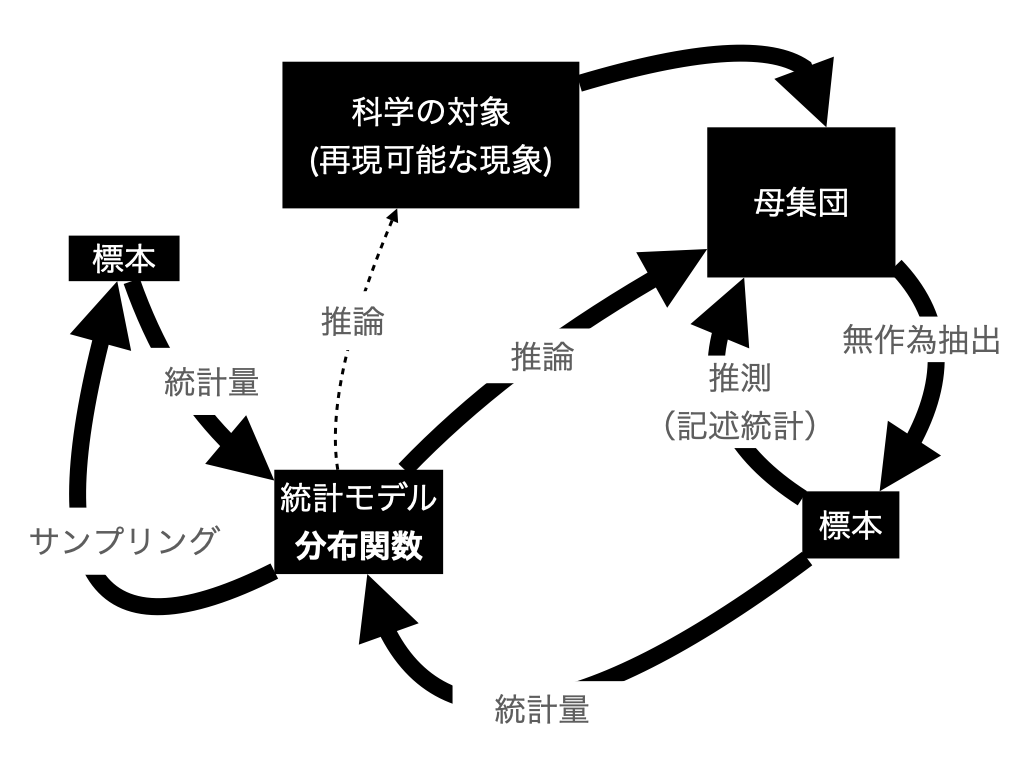
\includegraphics[bb=0 0 1024 768,width=15cm]{./image/01_/conceptual_diagram/conceptual_diagram.002.png}
  \caption{統計モデルによる現象の推測に関する概念図}
  \label{fig:conceptual_diagram_statistics}
 \end{center}
\end{figure}




%\subsection{適合しすぎな適合モデルは良いモデル?}%表現力・過学習・汎化性能}

\subsection{モデルの種類}
よく扱われるモデルを説明する。ただし、論文などではここでの説明通りにはなっていないことが多い。

データや数値を全く取り入れていないモデルをヌルモデルという。例えば、統計的仮説検定で出て来る統計モデルのいくつかは、データを取り入れない状態でもその統計的性質が判っており、その性質を使い、推論を行う。


ベースラインモデルは、既存のデータの一部およびモデルを使い、構築されたモデルのことである。
次のモデルをベースラインモデルと呼ぶことがある。
\begin{enumerate}
 \item データの平均値またはデータの一部を抜き出した何らかの定数。例えば$100$という値がデータに多く含まれていれば、$100$を予測値とするモデルをベースラインモデルとする。
 \item 過去の研究での最新のモデル。モデルの性能を比較するためにベースラインモデルとすることがある。
\end{enumerate}

\subsection{評価指標}
\subsubsection{$R^2$}
回帰分析では、平均値をもとにしたベースラインモデルと回帰モデルとの比較をおこなうため、$R^2$という指標が登場する。具体的には、次の形で回帰モデルの予測の良さを示す物である。

\begin{equation}
R^2 = 1- \frac{\sum (y_i-f(x_i))^2}{\sum (y_i-\bar{y})^2}
\end{equation}
ここで、$(x_i,y_i)$はデータ、$f(x_i)$は回帰モデルの予測、$\bar{y}$は、$y_i$の平均値である。分子は、回帰モデルとデータとの二乗誤差、分子は平近値を基にしたベースラインモデルとデータとの二乗誤差である。二つのモデルの二乗誤差を比較したものが$R^2$になっている。
モデルの上では、$R^2$は$0\sim 1$の値を取る。

データを入れた場合、
$R^2$が1に近ければ、回帰モデルの予測誤差が十分小さいことを示し、$R^2$が小くなると(負の値になることもある)、回帰モデルの予測誤差がベースラインモデルの予測誤差よりも大きい。
$R^2$が小さな値をとっているということは、回帰モデルよりも平近値を基にしたベースラインモデルの方が、平均二乗誤差の面で性能がよいことを示唆する。
%回帰モデルの場合、$R^2$は$0\sim 1$の値を取る

例えば、$R^2=0.25$であれば、
\begin{eqnarray*}
 \frac{\sum (y_i-f(x_i))^2}{\sum (y_i-\bar{y})^2} &=& 1-R^2 \\
 \rightarrow \sum (y_i-f(x_i))^2 &=& (1-R^2)\sum (y_i-\bar{y})^2 \\
 \rightarrow \sum (y_i-f(x_i))^2 &=& 0.75\sum (y_i-\bar{y})^2 \ \ (R^2 = 0.25を代入) \\
\end{eqnarray*}
と計算できる。
これを読み替えると、構築したモデル$f(x_i)$による予測と実際の差の二乗和、ベースラインモデルの誤差の二乗和を$2$割$5$分したものに等しいことがわかる\footnote{2乗和誤差$2$割$5$分引きのモデル}。
構築したモデルによる予測がベースラインモデルと比較して、相対的に良い予測をしていることを数値で示すことができる。


\section{疑似乱数}
乱数(でたらめな数)とは、人間の意図が加わらず、作為的でなく、規則性がなく、再現性もない数値列のことである。決定論を元に計算が行われているコンピュータ上では理想的な乱数列数を生成することできない。そこで、乱数の代わり擬似乱数を用いて、でたらめをまねた数値を生成することができる。

\subsection{逆関数法}
逆関数法は、ある確率密度関数$f(x)$に従う疑似乱数を生成する方法の一つである。
$f(x)$の累積分布関数を$F(x)$とする。$F(x)$は、値域を$[0,1]$にとる関数である。
このことから、$0\sim 1$の一様乱数$u$を生成し、累積分布関数の逆函數$x=F^{-1}(u)$を計算する。
すると、$x$は、確率密度関数$f(x)$に従う。

